\section{Result and Discussion}

\subsection{Experimental Setup}

All experiments in this section are controlled synthetic regression tasks, not LLM training runs. A frozen base weight $W_0 \in \mathbb{R}^{d\times k}$ is given together with a target update $\Delta W^{*}$, and the model learns $\Delta W$ so that $W_0+\Delta W$ approximates $W^{*}=W_0+\Delta W^{*}$. Because $\Delta W^{*}$ is known, the relative error $\|\hat{\Delta}-\Delta^{*}\|_F/\|\Delta^{*}\|_F$ can be measured directly. This isolates the low-rank hypothesis from confounders such as tokenizer, dataset, and prompt format, but it also means that every result below is a toy result and not evidence about LLM behaviour.

The training experiments use $d=k=256$ with fixed splits of 1024 training, 256 validation, and 256 test examples. The entries of $W_0$ are drawn from $\mathcal{N}(0,0.0625^2)$ and the observations are noise-free. The main target is \texttt{low\_rank} with true rank $r^{*}=8$, target noise $\sigma=0.01$, and scale ratio $\|\Delta W^{*}\|_F/\|W_0\|_F=0.5$. The limitation experiment (exp03) uses a full-rank \texttt{decaying\_spectrum} target with singular values proportional to $i^{-\gamma}$, for $\gamma\in\{0.5,1,2\}$.

All methods use Adam for 50 epochs with batch size 128 and weight decay $0$. The learning rate is selected from $\{0.001,0.01,0.1\}$ on the validation split; the selected rate is then used to report test metrics, so the test split is never used for model selection. Each configuration is run with five seeds $\{0,1,2,3,4\}$; a seed controls $W_0$, $\Delta W^{*}$, the data, and the initialization of the LoRA $A$ matrix. The compared methods are no fine-tuning ($\Delta W=0$), full fine-tuning (a dense trainable $\Delta W$ with the same parameter count as $W_0$), and LoRA with $r\in\{1,2,4,8,16\}$, $\alpha=16$, initialization standard deviation $0.01$, and $B=0$ at initialization.

Two optional experiments are also used. exp05 varies $r\in\{4,8\}$ and $\alpha\in\{4,8,16\}$ under validation-tuned and fixed (untuned) learning rates; the fixed rate is $0.03$. exp06 compares LoRA on the original base with LoRA on a simple absmax block 4-bit base (block size 64, 4 bits). The latter is a simulation and is \emph{not} NF4. The parameter and memory tables (exp01) are analytical calculations for a $1024\times1024$ layer; no training is involved.

The reported metrics are test mean squared error (MSE), relative delta error, trainable parameter count, and wall-clock training time. All runs were executed on Windows 11 with Python 3.10.19 and PyTorch 2.2.2+cu121 on an Intel Core i7-13700H (14 cores, 20 threads) and 32 GB of RAM. Only CPU execution was used; no GPU experimental results are claimed. The recorded commit for the result files is \texttt{6f47a47}.

\subsection{Parameter Efficiency Analysis}

Writing the adapted weight as $W'=W_0+\Delta W$ with $\Delta W=(\alpha/r)BA$, where $A\in\mathbb{R}^{r\times k}$ and $B\in\mathbb{R}^{d\times r}$, a layer of size $d\times k$ has $dk$ trainable parameters under full fine-tuning, whereas LoRA has $r(d+k)$ because only $A$ and $B$ are trained. For a $1024\times1024$ layer, full fine-tuning therefore has $1{,}048{,}576$ parameters, while LoRA with $r=4$, $8$, and $16$ has $8{,}192$, $16{,}384$, and $32{,}768$ parameters, respectively. These are $0.781\%$, $1.562\%$, and $3.125\%$ of the full count, corresponding to reductions of $128\times$, $64\times$, and $32\times$. In the $256\times256$ training runs, full fine-tuning has $65{,}536$ parameters and LoRA with $r=8$ has $4{,}096$.

\begin{table}[t]
\centering
\footnotesize
\setlength{\tabcolsep}{4pt}
\resizebox{\linewidth}{!}{%
\begin{tabular}{lrrrrrrr}
\toprule
Configuration & Trainable params & \% of full & Reduction & Weights (MiB) & Grads (MiB) & Adam (MiB) & Total (MiB) \\
\midrule
Full fine-tuning & 1{,}048{,}576 & 100.000\% & $1\times$ & 4.000 & 4.000 & 8.000 & 16.000 \\
LoRA $r=4$, $\alpha=16$ & 8{,}192 & 0.781\% & $128\times$ & 4.000 & 0.031 & 0.062 & 4.094 \\
LoRA $r=8$, $\alpha=16$ & 16{,}384 & 1.562\% & $64\times$ & 4.000 & 0.062 & 0.125 & 4.188 \\
LoRA $r=16$, $\alpha=16$ & 32{,}768 & 3.125\% & $32\times$ & 4.000 & 0.125 & 0.250 & 4.375 \\
\bottomrule
\end{tabular}
}
\caption{Trainable parameters and analytical memory estimate for one $1024\times1024$ layer (float32, Adam). The memory columns count frozen weights, gradients, and two Adam moments per trainable parameter; activations are excluded, so these are not measured GPU memory. Source: Team experiment (toy, synthetic), exp01.}
\label{tab:params_memory}
\end{table}


Table~\ref{tab:params_memory} also gives the analytical memory estimate for one $1024\times1024$ layer. For full fine-tuning, the frozen weights, gradients, and two Adam moments occupy 4 MiB, 4 MiB, and 8 MiB, respectively, for a total of 16 MiB. For LoRA with $r=4$, the corresponding total is 4.094 MiB; for $r=8$ and $r=16$ it is 4.188 MiB and 4.375 MiB. The frozen 4 MiB weight therefore dominates the estimate, while the gradient and optimizer terms shrink from 12 MiB combined to about 0.094 MiB at $r=4$. These values are analytical estimates that exclude activations and are not measured GPU memory; in particular, the trainable parameter count and GPU memory are different quantities.

The simulated 4-bit base in exp06 reduces base storage as well. For a $256\times256$ layer, the simple absmax block format occupies $36{,}864$ bytes, compared with $262{,}144$ bytes for the float32 base, a factor of about $7.1$. This count includes the per-block scales but excludes the adapter, gradients, optimizer state, and activations. It is a property of the simple quantizer used here, not of NF4.

\subsection{Experimental Results}

Figure~\ref{fig:rank_sweep} and Table~\ref{tab:rank_sweep} show the main rank sweep (exp02) on the rank-8 target. The no-fine-tuning baseline has test MSE $2.49\times10^{-1}$. Full fine-tuning reaches $6.15\times10^{-6}$. LoRA improves monotonically up to the true rank: test MSE is $2.06\times10^{-1}$ at $r=1$, $1.65\times10^{-1}$ at $r=2$, $1.01\times10^{-1}$ at $r=4$, $3.44\times10^{-6}$ at $r=8$, and $3.84\times10^{-6}$ at $r=16$. Ranks below $r^{*}=8$ therefore underfit strongly, and the sharp transition occurs exactly at $r=8$. Relative delta error follows the same pattern, from $9.09\times10^{-1}$ at $r=1$ to $3.72\times10^{-3}$ at $r=8$.

\begin{table}[t]
\centering
\footnotesize
\setlength{\tabcolsep}{4pt}
\resizebox{\linewidth}{!}{%
\begin{tabular}{lrrrr}
\toprule
Configuration & Trainable params & Test MSE & Rel. $\Delta$ error & Train time (s) \\
\midrule
No fine-tuning ($\Delta=0$) & 65{,}536 & $2.49\times 10^{-1}$ $\pm$ $1.35\times 10^{-2}$ & $1.00$ $\pm$ $0$ & $0.00 \pm 0.00$ \\
Full fine-tuning & 65{,}536 & $6.15\times 10^{-6}$ $\pm$ $2.69\times 10^{-6}$ & $4.90\times 10^{-3}$ $\pm$ $1.06\times 10^{-3}$ & $1.37 \pm 0.78$ \\
LoRA $r=1$, $\alpha=16$ & 512 & $2.06\times 10^{-1}$ $\pm$ $1.25\times 10^{-2}$ & $9.09\times 10^{-1}$ $\pm$ $5.69\times 10^{-3}$ & $0.70 \pm 0.06$ \\
LoRA $r=2$, $\alpha=16$ & 1{,}024 & $1.65\times 10^{-1}$ $\pm$ $1.36\times 10^{-2}$ & $8.17\times 10^{-1}$ $\pm$ $9.57\times 10^{-3}$ & $0.64 \pm 0.08$ \\
LoRA $r=4$, $\alpha=16$ & 2{,}048 & $1.01\times 10^{-1}$ $\pm$ $7.07\times 10^{-3}$ & $6.41\times 10^{-1}$ $\pm$ $5.42\times 10^{-3}$ & $0.70 \pm 0.04$ \\
LoRA $r=8$, $\alpha=16$ & 4{,}096 & $3.44\times 10^{-6}$ $\pm$ $2.15\times 10^{-7}$ & $3.72\times 10^{-3}$ $\pm$ $1.15\times 10^{-4}$ & $0.77 \pm 0.10$ \\
LoRA $r=16$, $\alpha=16$ & 8{,}192 & $3.84\times 10^{-6}$ $\pm$ $2.28\times 10^{-7}$ & $3.92\times 10^{-3}$ $\pm$ $1.16\times 10^{-4}$ & $0.90 \pm 0.07$ \\
\bottomrule
\end{tabular}
}
\caption{Rank sweep against full fine-tuning on the rank-8 synthetic target (mean $\pm$ sample std over five seeds). Learning rates are selected on the validation split and metrics are reported on the test split. CPU toy timings are not representative of LLM training. Source: Team experiment (toy, synthetic), exp02.}
\label{tab:rank_sweep}
\end{table}


In this setup, LoRA at $r=8$ is slightly better than full fine-tuning: test MSE $3.44\times10^{-6}$ versus $6.15\times10^{-6}$, and relative delta error $3.72\times10^{-3}$ versus $4.90\times10^{-3}$. Increasing the rank to $16$ does not improve the result and is slightly worse than $r=8$. This ordering is likely an optimization or regularization effect of the low-rank parameterization on this toy problem; it is not a general claim that LoRA outperforms full fine-tuning.

Figure~\ref{fig:fullrank} shows the full-rank target experiment (exp03). For $\gamma=0.5$, full fine-tuning reaches test MSE $9.65\times10^{-7}$ while the best LoRA configuration ($r=16$) reaches $1.15\times10^{-1}$, a gap of $+1.15\times10^{-1}$. For $\gamma=1$, the corresponding values are $9.73\times10^{-5}$ and $9.38\times10^{-3}$, a gap of $+9.29\times10^{-3}$. In both cases a small rank cannot represent the long spectral tail, which is the intended limitation. For $\gamma=2$, however, the target decays quickly enough that LoRA at $r=16$ reaches $4.18\times10^{-5}$ while full fine-tuning reaches $4.06\times10^{-4}$, so LoRA is better in this run. This exception does not support a universal ordering; it suggests that the effective rank of the target, rather than the label ``full-rank'', is the relevant quantity in this setup.

The merge check (exp04) compares the rank-$r$ forward path with the merged dense layer on a test batch. The maximum absolute error over five seeds is $5.25\times10^{-6}$ for full fine-tuning, $4.77\times10^{-6}$ for LoRA at $r=4$, $4.29\times10^{-6}$ at $r=8$, and $4.53\times10^{-6}$ at $r=16$. All values are below the configured threshold of $10^{-5}$, so the merged layer is numerically equivalent to the adapter path within float32 tolerance; the merge errors are included in Table~\ref{tab:comparison}.

Figure~\ref{fig:alpha} summarises the $\alpha$-scaling experiment (exp05). At $r=8$ with validation-tuned learning rates, $\alpha=4$, $8$, and $16$ give test MSE $3.02\times10^{-6}$, $3.10\times10^{-6}$, and $3.44\times10^{-6}$. With the fixed learning rate, the same settings give $6.31\times10^{-6}$, $2.31\times10^{-5}$, and $4.14\times10^{-4}$. At $r=4$, all settings remain near $1.0\times10^{-1}$. Thus $\alpha$ and the learning rate interact: validation tuning narrows the gap between $\alpha$ values, while a large $\alpha$ with a fixed rate degrades the result.

\begin{figure}[t]
\centering
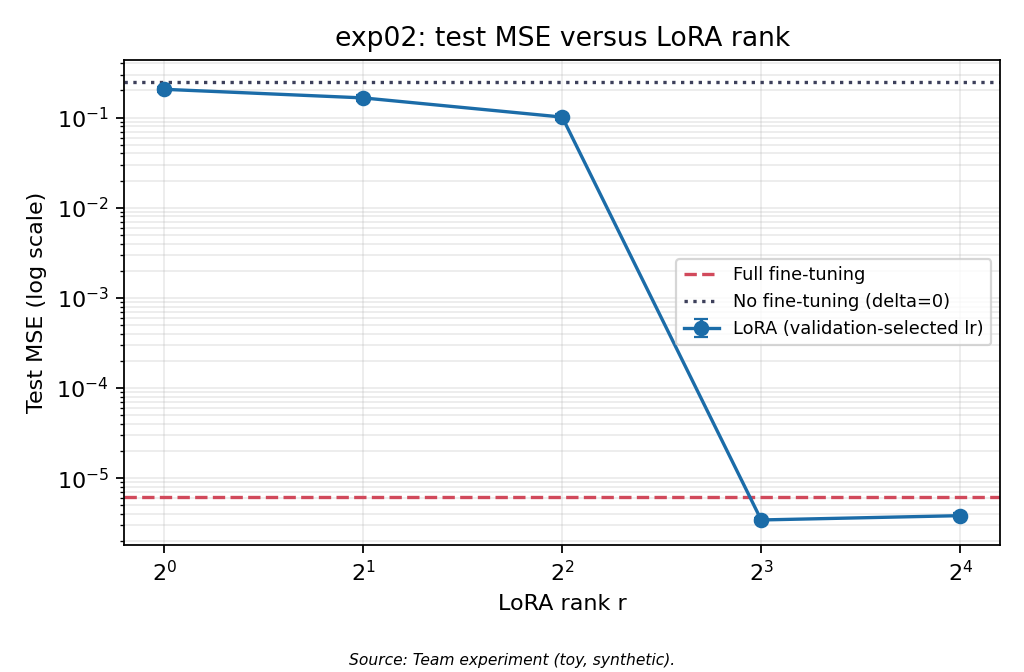
\includegraphics[width=\linewidth]{figures/rank_sweep.png}
\caption{Test MSE versus LoRA rank on the rank-8 synthetic target (exp02). The dashed line is full fine-tuning and the dotted line is no fine-tuning. Markers are means over five seeds; the vertical axis is logarithmic. Source: Team experiment (toy, synthetic).}
\label{fig:rank_sweep}
\end{figure}

\begin{figure}[t]
\centering
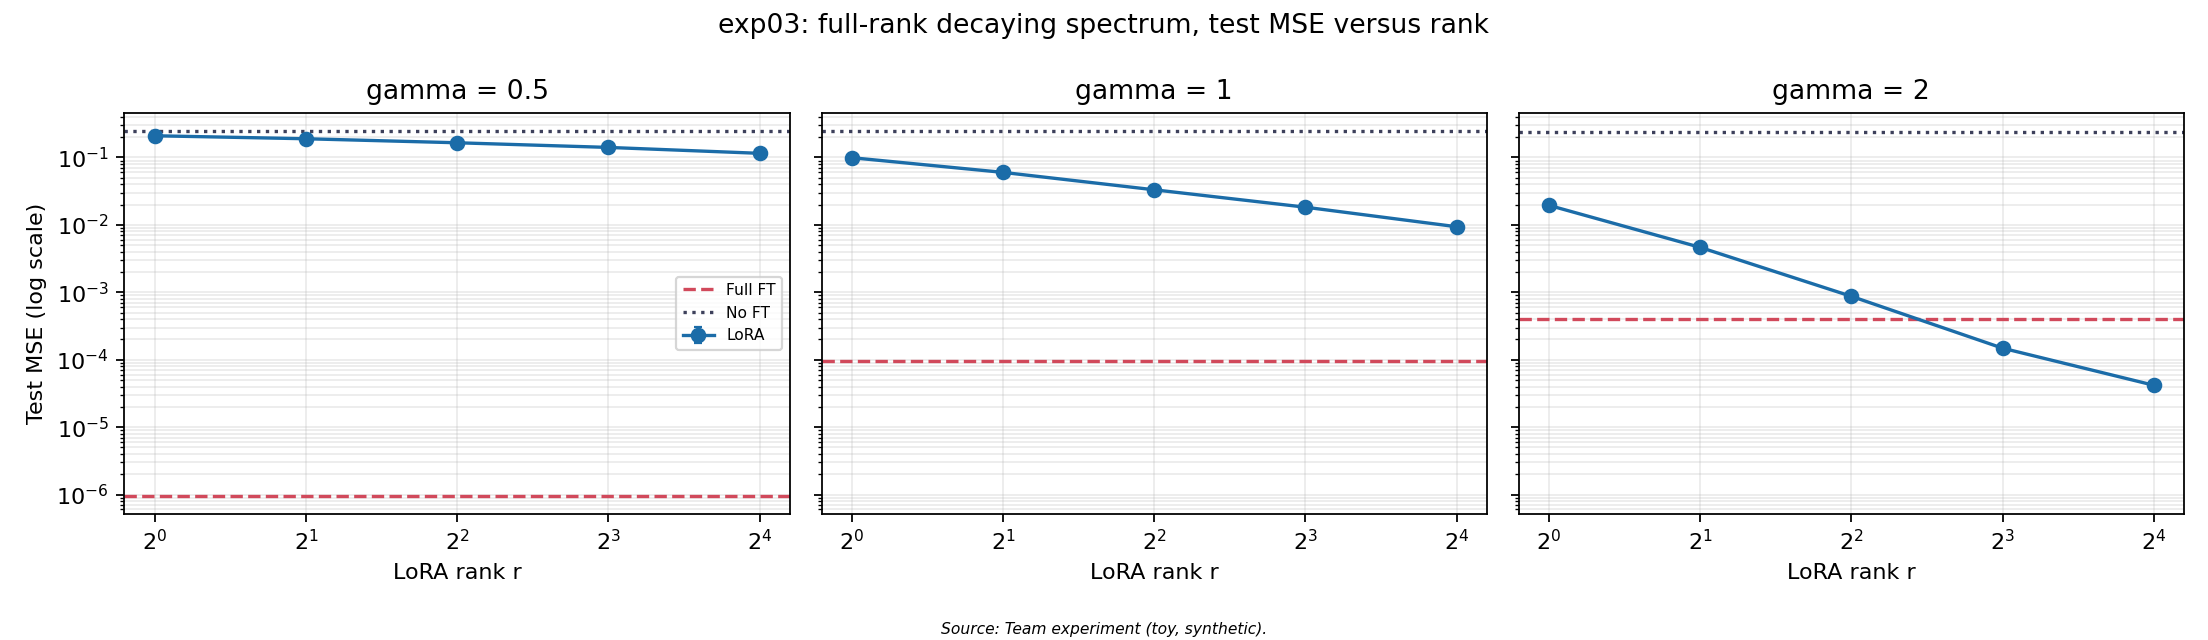
\includegraphics[width=\linewidth]{figures/fullrank.png}
\caption{Test MSE versus LoRA rank for the full-rank decaying-spectrum targets with $\gamma\in\{0.5,1,2\}$ (exp03). Dashed lines are full fine-tuning and dotted lines are no fine-tuning. Markers are means over five seeds; the vertical axis is logarithmic. Source: Team experiment (toy, synthetic).}
\label{fig:fullrank}
\end{figure}

\begin{figure}[t]
\centering
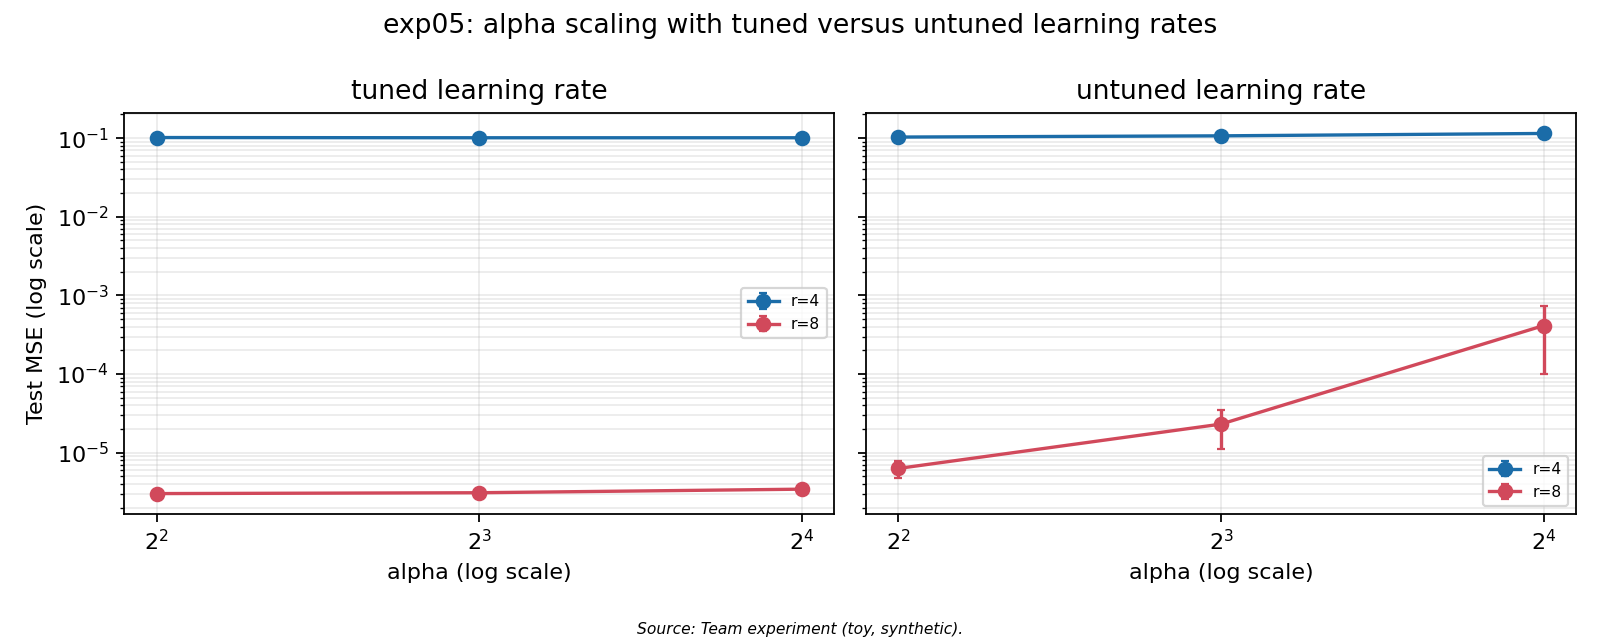
\includegraphics[width=\linewidth]{figures/alpha_scaling.png}
\caption{Test MSE for the $\alpha$-scaling configurations (exp05) with validation-tuned and fixed (untuned) learning rates. The figure reports means over five seeds. Source: Team experiment (toy, synthetic).}
\label{fig:alpha}
\end{figure}

\subsection{LoRA vs. QLoRA vs. Full Fine-Tuning}

Table~\ref{tab:comparison} compares full fine-tuning, LoRA at $r=4$, $8$, and $16$, and the simulated 4-bit-base variants on the same synthetic target. Full fine-tuning trains $65{,}536$ parameters; LoRA at $r=8$ trains $4{,}096$, which is $6.25\%$ of the full count and $16\times$ fewer parameters in this $256\times256$ layer (the corresponding reduction for a $1024\times1024$ layer is $64\times$). The test errors are those discussed above: full fine-tuning $6.15\times10^{-6}$, LoRA at $r=8$ $3.44\times10^{-6}$, and LoRA at $r=4$ $1.01\times10^{-1}$.

\begin{table}[t]
\centering
\footnotesize
\setlength{\tabcolsep}{4pt}
\resizebox{\linewidth}{!}{%
\begin{tabular}{lrrrrrrr}
\toprule
Configuration & Trainable params & Test MSE & Rel. $\Delta$ error & Base (KiB) & Quant. error & Train time (s) & Merge err. \\
\midrule
Full FT (float32) & 65{,}536 & $6.15\times 10^{-6}$ $\pm$ $2.69\times 10^{-6}$ & $4.90\times 10^{-3}$ $\pm$ $1.06\times 10^{-3}$ & 256 & 0 & $1.37 \pm 0.78$ & $5.25\times 10^{-6}$ \\
LoRA $r=4$ (float32) & 2{,}048 & $1.01\times 10^{-1}$ $\pm$ $7.07\times 10^{-3}$ & $6.41\times 10^{-1}$ $\pm$ $5.42\times 10^{-3}$ & 256 & 0 & $0.70 \pm 0.04$ & $4.77\times 10^{-6}$ \\
LoRA $r=8$ (float32) & 4{,}096 & $3.44\times 10^{-6}$ $\pm$ $2.15\times 10^{-7}$ & $3.72\times 10^{-3}$ $\pm$ $1.15\times 10^{-4}$ & 256 & 0 & $0.77 \pm 0.10$ & $4.29\times 10^{-6}$ \\
LoRA $r=16$ (float32) & 8{,}192 & $3.84\times 10^{-6}$ $\pm$ $2.28\times 10^{-7}$ & $3.92\times 10^{-3}$ $\pm$ $1.16\times 10^{-4}$ & 256 & 0 & $0.90 \pm 0.07$ & $4.53\times 10^{-6}$ \\
Full FT + 4-bit base (sim.) & 65{,}536 & $6.70\times 10^{-6}$ $\pm$ $2.89\times 10^{-6}$ & $1.98\times 10^{-1}$ $\pm$ $1.02\times 10^{-3}$ & 36 & $9.92\times 10^{-2}$ & $1.01 \pm 0.08$ & n/a \\
LoRA $r=8$ + 4-bit base (sim.) & 4{,}096 & $9.32\times 10^{-3}$ $\pm$ $1.34\times 10^{-4}$ & $5.26\times 10^{-2}$ $\pm$ $7.16\times 10^{-4}$ & 36 & $9.92\times 10^{-2}$ & $0.72 \pm 0.05$ & n/a \\
\bottomrule
\end{tabular}
}
\caption{Comparison of full fine-tuning, LoRA, and simulated 4-bit-base variants on the synthetic target (mean $\pm$ sample std over five seeds). ``Base'' is the stored size of one $256\times256$ frozen base and excludes adapters, gradients, optimizer state, and activations. Merge error is the maximum over seeds (threshold $10^{-5}$). The 4-bit rows use simple absmax block quantization, \emph{not} NF4. Source: Team experiment (toy, synthetic), exp02/exp04/exp06.}
\label{tab:comparison}
\end{table}


The 4-bit rows use the simple absmax block quantizer, not NF4. The mean quantization error is $9.92\times10^{-2}$. LoRA at $r=8$ on the 4-bit base reaches test MSE $9.32\times10^{-3}$ and relative delta error $5.26\times10^{-2}$, versus $3.44\times10^{-6}$ and $3.72\times10^{-3}$ for the float32 base. Full fine-tuning on the 4-bit base reaches test MSE $6.70\times10^{-6}$ but relative delta error $1.98\times10^{-1}$, compared with $4.90\times10^{-3}$ on the float32 base. A dense adapter can therefore compensate for part of the quantization error in output space, while the recovered weight update differs substantially from the target. This simulation does not establish that QLoRA recovers the original model, and it is not an NF4 experiment.

The definitions of LoRA and QLoRA follow the original papers \cite{hu2022lora,dettmers2023qlora}: LoRA freezes the base weight and learns a low-rank update, and QLoRA combines a frozen quantized base with high-precision low-rank adapters. All numerical statements in this section are team measurements from the toy experiments; no quantitative LLM result is taken from either paper.

\subsection{Practical Trade-offs}

The results suggest several trade-offs. First, quality depends strongly on the rank relative to the effective rank of the target. In exp02, ranks below $r^{*}=8$ underfit, while $r=16$ gives no improvement over $r=8$. In exp03, a long spectral tail at $\gamma=0.5$ and $\gamma=1$ is not representable at small rank, whereas the quickly decaying target at $\gamma=2$ is.

Second, memory savings are real but narrower than the parameter ratio suggests. For the $1024\times1024$ layer, LoRA reduces the analytical total from 16 MiB to about 4.1--4.4 MiB, but the frozen 4 MiB base remains. QLoRA reduces the base storage further, to about $36$ KiB versus $256$ KiB for a $256\times256$ layer in the simulation, at the cost of a measurable quantization error. Activations, which are excluded from all estimates here, can dominate real training memory and are not reduced by LoRA in the same way.

Third, training time is lower for LoRA in this toy setting: about $0.70$--$0.90$ s versus $1.37$ s for full fine-tuning over five seeds. These are CPU toy timings and are not representative of LLM training. Fourth, inference can be made equivalent to the base model: merging produces a single dense layer, and the merge check in Table~\ref{tab:comparison} is below $10^{-5}$. Keeping the adapter unmerged preserves the ability to swap adapters at inference time.

Fifth, $\alpha$ and the learning rate interact. In exp05, validation tuning makes $\alpha=4$, $8$, and $16$ nearly equivalent at $r=8$, while a fixed rate makes larger $\alpha$ clearly worse. This is consistent with the view that $\alpha/r$ rescales the update and therefore changes the effective learning rate.

Finally, LoRA may not be the best choice when the update has high intrinsic rank or a long spectral tail (as in exp03 at $\gamma=0.5$ and $\gamma=1$), when the model is small enough that full fine-tuning is cheap, or when the distribution shift is large; the last case was not tested here. The $\gamma=2$ result is a reminder that the relevant condition is the effective rank of the update, not a binary full-rank label.

\subsection{Limitations and Experimental Risks}

The main limitation is the synthetic, single-layer linear setting. The data, the base weight, and the target are generated, and the scale is far below any LLM. CPU toy timings are not representative of real training hardware. The QLoRA experiment is a simple 4-bit absmax simulation, not NF4, and it does not reproduce the QLoRA training pipeline; its conclusions should not be transferred to LLMs. The optional PEFT DistilBERT/SST-2 experiment (exp07) was not run because it requires a GPU and the optional Hugging Face dependencies, so no DistilBERT or SST-2 results are claimed.

The statistical basis is also limited: five seeds and a coarse learning-rate grid, with results that depend on $\alpha$, initialization, and the chosen $r^{*}$. The conclusions are conditional on this model class and optimizer. There is a risk of overfitting the interpretation to the chosen true rank of $8$, and the unexpected orderings in exp02 and exp03 ($\gamma=2$) show that optimization effects can be as important as representational ones. All text in this section was drafted with AI assistance and should be independently checked against the generated tables and figures.

In summary, the results support the following statements in this setup: LoRA with $r\approx r^{*}$ matches or slightly exceeds full fine-tuning with far fewer trainable parameters; ranks below the true rank underfit a low-rank target; small ranks cannot represent a long spectral tail; merging is numerically equivalent to the adapter path; and a simple 4-bit base introduces a measurable error. They do not support general claims about LLM fine-tuning, NF4 performance, or universal superiority of any method.
